\question{Спонтанные и индуцированные переходы. Коэффициенты Эйнштейна.}

\subquestion{Спонтанные и индуцированные переходы}

\emph{Спонтанные переходы} -- самопроизвольные переходы квантовой систем 
из состояния с высокой энергией в состояние с низкой энергией.

\emph{Вынужденные переходы} -- переходы между уровнями энергии квантовой 
системы под действием внешнего излучения, энергия квантов которого равна 
разнице уровней. В отличие от спонтанного, происходит как сверху вниз, так 
и снизу вверх и зависит от интенсивности внешнего излучения.

\question{Коэффициенты Эйнштейна}

\begin{figure}[h!]
	\center
	%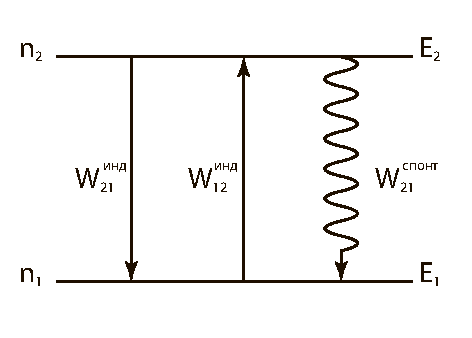
\includegraphics[width=.4\textwidth]{image1_1} \\
	%\caption{Схема двух уровней энергии \( E_2 > E_1 \)}
	\label{img1.1}
\end{figure}

\( A_{21} \) -- это вероятность самопроизвольного перехода из состояния 
\( 2 \) в состояние \( 1 \) в единицу времени. 

\( B_{12} \), \( B_{21} \) -- вероятность вынужденного перехода 
\( 1 \leftarrow 2 \) (\( 2 \leftarrow 1 \)) в единицу времени, отнесённая к 
спектральной объёмной плотности излучения \( \rho_\nu \).